\documentclass[11pt,openany]{article}

\usepackage{mathtools, commath}
% Packages for formatting
\usepackage[margin=1in]{geometry}
\usepackage{fancyhdr}
\usepackage{enumerate}
\usepackage{graphicx}
\usepackage{kotex}
\usepackage{arydshln} % Include this package
\usepackage{bbding}
\usepackage{amsmath}
\usepackage{amsthm}
\usepackage[dvipsnames,table]{xcolor}
\usepackage{amssymb, amsfonts}
\usepackage{wasysym}
\usepackage{footnote}
\usepackage{tablefootnote}
\usepackage{arydshln} % Include this package
% Fonts
\usepackage[T1]{fontenc}
\usepackage[utf8]{inputenc}
\usepackage{newpxtext,newpxmath}
\usepackage{sectsty}

% Define colors
\definecolor{TealBlue1}{HTML}{0077c2}
\definecolor{TealBlue2}{HTML}{00a5e6}
\definecolor{TealBlue3}{HTML}{b3e0ff}
\definecolor{TealBlue4}{HTML}{00293c}
\definecolor{TealBlue5}{HTML}{e6f7ff}

\definecolor{thmcolor}{RGB}{231, 76, 60}
\definecolor{defcolor}{RGB}{52, 152, 219}
\definecolor{lemcolor}{RGB}{155, 89, 182}
\definecolor{corcolor}{RGB}{46, 204, 113}
\definecolor{procolor}{RGB}{241, 196, 15}

\usepackage{color,soul}
\usepackage{soul}
\newcommand{\mathcolorbox}[2]{\colorbox{#1}{$\displaystyle #2$}}
\usepackage{cancel}
\newcommand\crossout[3][black]{\renewcommand\CancelColor{\color{#1}}\cancelto{#2}{#3}}
\newcommand\ncrossout[2][black]{\renewcommand\CancelColor{\color{#1}}\cancel{#2}}

\usepackage{hyperref}
\usepackage{booktabs}

% Chapter formatting
\definecolor{titleTealBlue}{RGB}{0,53,128}
\usepackage{titlesec}
\titleformat{\section}
{\normalfont\sffamily\Large\bfseries\color{titleTealBlue!100!gray}}{\thesection}{1em}{}
\titleformat{\subsection}
{\normalfont\sffamily\large\bfseries\color{titleTealBlue!50!gray}}{\thesubsection}{1em}{}

%Tcolorbox
\usepackage[most]{tcolorbox}
\usepackage{multirow}
\usepackage{multicol}

\usepackage[linesnumbered,ruled]{algorithm2e}
\usepackage{algpseudocode}
\usepackage{setspace}
\SetKwComment{Comment}{/* }{ */}
\SetKwProg{Fn}{Function}{:}{end}
\SetKw{End}{end}
\SetKw{DownTo}{downto}

% Define a new environment for algorithms without line numbers
\newenvironment{algorithm2}[1][]{
	% Save the current state of the algorithm counter
	\newcounter{tempCounter}
	\setcounter{tempCounter}{\value{algocf}}
	% redefine the algorithm numbering (remove prefix)
	\renewcommand{\thealgocf}{}
	\begin{algorithm}
	}{
	\end{algorithm}
	% Restore the algorithm counter state
	\setcounter{algocf}{\value{tempCounter}}
}

\usepackage{adjustbox}
% Header and footer formatting
\pagestyle{fancy}
\fancyhead{}
\fancyhf{}
\rhead{\textcolor{TealBlue2}{\large\textbf{기대수(기초부터 대학원 수학까지 시리즈) 3기}}}%\rule{3cm}{0.4pt}}
\lhead{\textcolor{TealBlue2}{\large\textbf{수학의 즐거움, Enjoying Math}}}
% Define footer
%\newcommand{\footer}[1]{
%\begin{flushright}
%	\vspace{2em}
%	\includegraphics[width=2.5cm]{school_logo.jpg} \\
%	\vspace{1em}
%	\textcolor{TealBlue2}{\small\textbf{#1}}
%\end{flushright}
%}
%\rfoot{\large Department of Information Security, Cryptogrphy and Mathematics, Kookmin Uni.\includegraphics[height=1.5cm]{school_logo.jpg}}
\fancyfoot{}
\fancyfoot[C]{-\thepage-}

\usepackage{tcolorbox}
\tcbset{colback=white, arc=5pt}

\definecolor{axiomcolor}{HTML}{a88bfa}
\definecolor{defcolor}{RGB}{52, 152, 219}
\definecolor{procolor}{RGB}{241, 196, 15}
\definecolor{thmcolor}{RGB}{231, 76, 60}
\definecolor{lemcolor}{RGB}{155, 89, 182}
\definecolor{corcolor}{RGB}{46, 204, 113}
\definecolor{execolor}{RGB}{90, 128, 127}

% Define a new command for the custom tcolorbox
\newcommand{\axiombox}[2][]{%
	\begin{tcolorbox}[colframe=axiomcolor, title={\color{white}\bfseries #1}]
		#2
	\end{tcolorbox}
}

\newcommand{\defbox}[2][]{%
	\begin{tcolorbox}[colframe=defcolor, title={\color{white}\bfseries #1}]
		#2
	\end{tcolorbox}
}

\newcommand{\lembox}[2][]{%
	\begin{tcolorbox}[colframe=lemcolor, title={\color{white}\bfseries #1}]
		#2
	\end{tcolorbox}
}

\newcommand{\probox}[2][]{%
	\begin{tcolorbox}[colframe=procolor, title={\color{white}\bfseries #1}]
		#2
	\end{tcolorbox}
}

\newcommand{\thmbox}[2][]{%
	\begin{tcolorbox}[colframe=thmcolor, title={\color{white}\bfseries #1}]
		#2
	\end{tcolorbox}
}

\newcommand{\corbox}[2][]{%
	\begin{tcolorbox}[colframe=corcolor, title={\color{white}\bfseries #1}]
		#2
	\end{tcolorbox}
}



\usepackage{amsthm}

% Define custom theorem styles
\newtheoremstyle{dotless} % Name of the style
{3pt} % Space above
{3pt} % Space below
{\itshape} % Body font
{} % Indent amount
{\bfseries} % Theorem head font
{} % Punctuation after theorem head
{2.5mm} % Space after theorem head
{} % Theorem head spec

\newtheoremstyle{definitionstyle} % Name of the style
{3pt} % Space above
{3pt} % Space below
{} % Body font
{} % Indent amount
{\bfseries} % Theorem head font
{.} % Punctuation after theorem head
{2.5mm} % Space after theorem head
{} % Theorem head spec

% Applying custom styles
\theoremstyle{dotless}
\newtheorem{theorem}{Theorem} % Theorem environment with section-wise numbering
\newtheorem{proposition}[theorem]{Proposition} % Theorem environment with section-wise numbering
\newtheorem{lemma}[theorem]{Lemma} % Lemma shares the counter with theorem
\newtheorem{corollary}[theorem]{Corollary} % Corollary shares the counter with theorem

\theoremstyle{definitionstyle}
\newtheorem*{observation}{\textcolor{Magenta}{Observation}}
\newtheorem{definition}{Definition} % Definition shares the counter with theorem
\newtheorem{example}{Example} % Example shares the counter with theorem
\newtheorem{exercise}{Exercise} % Example shares the counter with theorem
\newtheorem{remark}{Remark} % Remark shares the counter with theorem
\newtheorem*{note}{Note}

\newtheorem*{definition*}{Definition} % Definition shares the counter with theorem
\newtheorem*{example*}{Example} % Example shares the counter with theorem
\newtheorem*{exercise*}{\textcolor{violet}{Exercise}} % Example shares the counter with theorem
\newtheorem*{remark*}{Remark} % Remark shares the counter with theorem


\usepackage{tikz}
\usepackage{tikz-cd}
\usepackage{tikz-3dplot}
\usepackage{pgfplots}
\pgfplotsset{compat=newest} % Adjust to your version of pgfplots
\def\Circlearrowleft{\ensuremath{%
		\rotatebox[origin=c]{180}{$\circlearrowleft$}}}
\def\Circlearrowright{\ensuremath{%
		\rotatebox[origin=c]{180}{$\circlearrowright$}}}
\def\CircleArrowleft{\ensuremath{%
		\reflectbox{\rotatebox[origin=c]{180}{$\circlearrowleft$}}}}
\def\CircleArrowright{\ensuremath{%
		\reflectbox{\rotatebox[origin=c]{180}{$\circlearrowright$}}}}
\usetikzlibrary{
	3d, % For 3D drawing
	angles,
	arrows,
	arrows.meta,
	backgrounds,
	bending,
	calc,
	decorations.pathmorphing,
	decorations.pathreplacing,
	decorations.markings,
	fit,
	matrix,
	patterns,
	patterns.meta,
	positioning,
	quotes,
	shadows,
	shapes,
	shapes.geometric,
	tikzmark
}
\tikzset{
	% single mid‐path arrow
	mid arrow/.style={
		decoration={
			markings,
			mark=at position 0.5 with {\arrow{Stealth[scale=1.2]}}
		},
		postaction={decorate},
	},
	% style for field arrows
	field arrow/.style={
		-{Stealth[scale=1.0]},
		thick,
		blue!70!black,
	},
}
\newcommand{\ie}{\textnormal{i.e.}}
\newcommand{\rsa}{\mathsf{RSA}}
\newcommand{\rsacrt}{\mathsf{RSA}\textendash\mathsf{CRT}}
\newcommand{\inv}[1]{#1^{-1}}

%New Command
%\newcommand{\set}[1]{\left\{#1\right\}}
\newcommand{\N}{\mathbb{N}}
\newcommand{\Z}{\mathbb{Z}}
\newcommand{\Q}{\mathbb{Q}}
\newcommand{\R}{\mathbb{R}}
\newcommand{\cR}{\mathcal{R}}
\newcommand{\C}{\mathbb{C}}
\newcommand{\F}{\mathbb{F}}
\newcommand{\nbhd}{\mathcal{N}}
\newcommand{\Log}{\operatorname{Log}}
\newcommand{\Arg}{\operatorname{Arg}}
\newcommand{\pv}{\operatorname{P.V.}}

\newcommand{\of}[1]{\left( #1 \right)} 
%\newcommand{\abs}[1]{\left\lvert #1 \right\rvert}
%\newcommand{\norm}[1]{\left\| #1 \right\|}

\newcommand{\sol}{\textcolor{magenta}{\bf Sol}}
\newcommand{\conjugate}[1]{\overline{#1}}

\newcommand{\res}{\operatorname{res}}
\DeclareMathOperator*{\Res}{\operatorname{Res}}

%\renewcommand{\Re}{\operatorname{Re}}
%\renewcommand{\Im}{\operatorname{Im}}

\newcommand{\cyclic}[1]{\langle #1 \rangle}
\newcommand{\uniform}{\overset{\$}{\leftarrow}}
\newcommand{\xmark}{\textcolor{red}{\XSolidBrush}}
\newcommand{\vmark}{\textcolor{green!75!black}{\CheckmarkBold}}

\newcommand{\gen}[1]{\langle #1 \rangle}
\newcommand{\Gen}[1]{\left\langle #1 \right\rangle}

\newcommand{\img}[1]{\text{Img}(#1)}
\newcommand{\Img}[1]{\text{Img}\left(#1\right)}
\newcommand{\preimg}[1]{\text{Img}^{-1}(#1)}
\newcommand{\Preimg}[1]{\text{Img}^{-1}\left(#1\right)}

\newcommand{\relation}{\mathrel{\mathcal{R}}}
\newcommand{\injection}{\rightarrowtail}
\newcommand{\surjection}{\twoheadrightarrow}
\newcommand{\id}{\textnormal{id}}

\newcommand{\eqclass}[1]{\left[#1\right]}

% Define custom colors for O and X
\newcommand{\yes}{\textcolor{blue}{\bf \fullmoon}}
\newcommand{\no}{\textcolor{red}{\bf \texttimes}}

\DeclarePairedDelimiter\ceil{\lceil}{\rceil}
\DeclarePairedDelimiter\floor{\lfloor}{\rfloor}
%\renewcommand{\floor}[#1]{\lfloor #1\rfloor}
%\newcommand{\Floor}[#1]{\left\lfloor #1\right\rfloor}
%\newcommand{\ceil}[#1]{\lceil #1\rceil}
%\newcommand{\Ceil}[#1]{\left\lceil #1\right\rceil}

\newcommand{\topology}{\mathscr{T}}
\newcommand{\sequence}[1]{\langle #1\rangle}
\renewcommand{\vec}[1]{\mathbf{#1}}
\renewcommand{\Re}{\operatorname*{Re}}
\renewcommand{\Im}{\operatorname*{Im}}
\setstretch{1.25}

%\usepackage{background}
%\backgroundsetup{
%	scale=3,
%	color=gray!20,
%	opacity=0.3,
%	angle=45,
%	contents={\Huge \sffamily Ji, Yong-hyeon}
%}
\begin{document}
\pagenumbering{arabic}
\begin{center}
	\huge\textbf{Abstract Algebra I}\\
	\vspace{0.5em}
	\large{Ji, Yong-hyeon}\\
%	\large{\ttfamily \url{https://github.com/Hacker-Code-J}}\\
	\vspace{0.5em}
	\normalsize{\today}\\
\end{center}

\noindent 
We cover the following topics in this note.
\begin{itemize}
	\item Cyclic Group
	\item Classification of Cyclic Group
	\item Order of an Element
	\item Converge of Lagrange's Theorem
	\item Coset
	\item Lagrange's Theorem
\end{itemize}
\hrule\vspace{12pt}
\tableofcontents


\newpage
\section*{Cyclic Group and its Classification}
\addcontentsline{toc}{section}{Cyclic Group and its Classification}
%We develop the concept of cyclic groups and establish their complete classification.
\begin{note}
Let \( (G, \ast) \) be a group with identity element \( e \). Recall that the axioms of a group require:
\begin{enumerate}[(G1)]
	\item[] (G0)\; $\forall\, x, y \in G,\;  x \ast y\in G$;
	\item[] (G1)\; $\forall\, x, y, z \in G,\;  (x \ast y) \ast z = x \ast (y\ast z)$;
	\item[] (G2)\; $\exists\, e \in G,\; \text{s.t.}\; \forall\, x \in G,\; e \cdot x = x \cdot e = x$;
	\item[] (G3)\; $\forall\, x \in G,\; \exists\, x^{-1} \in G\; \text{s.t.}\; x \cdot x^{-1} = x^{-1} \cdot x = e$.
\end{enumerate}
%Consider \((\mathbb{Z},+)\) as the additive group of integers. For \( a \in G \) and \( n \in \mathbb{Z} \), the notation
%\[
%a^n \coloneqq
%\begin{cases}
%	\underbrace{a \ast a \ast \cdots \ast a}_{n \text{ times}} &: n > 0, \\
%	e &: n = 0, \\
%	(a^{-1})^{-n}&: n < 0,
%\end{cases}
%\]
%defines the \( n \)-th power of \( a \).
\end{note}
\defbox[Cyclic Group]{\begin{definition*}
	A group $G$ is said to be \textbf{cyclic} if and only if \[
	\exists\, a \in G \;\text{such that}\; \Bigl[\, \forall\, g \in G,\; \exists\, n \in \mathbb{Z} \text{ with } g = a^n \Bigr].
	\] The element \( a \) is called a \textbf{generator} of \( G \).
\end{definition*}}
\begin{remark*}
	The notation \(a^n\) (or $na$) is understood in the group-theoretic sense, \[
	a^n \coloneqq
	\begin{cases}
		\underbrace{a \ast \cdots \ast a}_{\abs{n}=n \text{ factors}} &: n > 0, \\
		e_G &: n = 0, \\
		\underbrace{(a^{-1})\ast\cdots\ast (a^{-1})}_{\abs{n}=-n\; \text{factors}}=(a^{-1})^{-n}&: n < 0,
	\end{cases}\quad\quad\text{or}\quad\quad	
na \coloneqq
\begin{cases}
\underbrace{a \ast \cdots \ast a}_{\abs{n}=n \text{ factors}} &: n > 0, \\
e_G &: n = 0, \\
\underbrace{(-a)\ast\cdots\ast a^{-1}}_{\abs{n}=-n \text{ factors}}=(-n)(-a)&: n < 0.
\end{cases}
\] Note that for all $m,n\in\Z$, \[
g^{m+n}=g^m\ast g^n\quad\text{(or $(m+n)g=mg\ast ng$)}.
\]
%We wish to show that for all \(m, n\in\Z\), \[
%g^{m+n} = g^m \ast g^n.
%\]
%\textbf{Case 1.} (\(m,n \ge 0\)); We prove by induction on \(n\) that \(g^{m+n} = g^m \cdot g^n\) for any fixed \(m \ge 0\).
%\begin{enumerate}[(i)]
%	\item Basic Step.\; Let $n=0$. Then $g^{m+0}=g^m = g^m\ast e=g^m\ast g^0$.
%	\item Inductive Step.\; Assume that for some \(n \ge 0\), $g^{m+n} = g^m \ast g^n$. Then \begin{align*}
%		g^{m+(n+1)} = g^{(m+n)+1} &= g^{m+n} \ast g\\
%		&=\bigl( g^m \ast g^n \bigr) \ast g\quad\text{by the induction hypothesis}\\
%		&=g^m\ast \bigl(g^n\ast g\bigr) \\
%		&=g^m\ast g^{n+1}.
%	\end{align*}
%\end{enumerate}
%\textbf{Case 2.} \(m,n \le 0\).\\
%Let \(m = -p\) and \(n = -q\) with \(p,q \ge 0\). By the definition, we have \[
%g^m=g^{-p}=(g^{-1})^{-(-p)}=(g^{-1})^p,\quad g^n=g^{-q}=(g^{-1})^{-(-q)}=(g^{-1})^q.
%\]Then, \begin{align*}
%g^{m+n} = g^{-p - q} =g^{-(p+q)} &= \bigl( g^{-1} \bigr)^{p+q}.\\
%&=\bigl( g^{-1}\bigr)^{p}\ast\bigl( g^{-1}\bigr)^{q}\quad\text{by Case 1}\\
%&=g^m\ast g^n.
%\end{align*}
%\textbf{Case 3.} Without loss of generality, \(m \ge 0\) and \(n < 0\). \\
%Write \(n = -q\) with \(q \ge 0\). Consider\[
%g^{m+n}=g^{m+( - q)}.
%\]
%\begin{itemize}
%	\item {3--(a)}\; Let \(m \ge q\). Then  \[
%	g^m = g^{(m - q) + q} = g^{m-q} \ast g^q=g^m\ast (g^{-1})^q.
%	\]
%	Multiplying on the right by \((g^q)^{-1}\) (which is \(g^{-q}\)) yields:
%	\[
%	g^{m-q} = g^m \cdot (g^q)^{-1} = g^m \cdot g^{-q}.
%	\] {3--(b)}\; Let \(m < q\).
%	Then \(m - q < 0\) and we write
%	\[
%	g^{m-q} = \bigl( g^{q-m} \bigr)^{-1}.
%	\]
%	By Case 1,
%	\[
%	g^q = g^m \cdot g^{q-m}.
%	\]
%	Taking inverses gives:
%	\[
%	g^{-q} = \bigl( g^m \cdot g^{q-m} \bigr)^{-1} = \bigl( g^{q-m} \bigr)^{-1} \cdot (g^m)^{-1} = g^{m-q} \cdot g^{-m}.
%	\]
%	Then multiplying on the right by \(g^m\) yields:
%	\[
%	g^{m-q} = g^{-q} \cdot g^m.
%	\]
%\end{itemize}
%Thus, in all cases, we conclude that for every \(m,n \in \mathbb{Z}\),
%\[
%g^{m+n} = g^m \cdot g^n.
%\]
\end{remark*}

\newpage
\thmbox[The Classification for Cyclic Groups]{\begin{theorem*}
Let \((G,\ast)\) be a cyclic group. Then
\[
(G,\ast) \simeq
\begin{cases}
	(\mathbb{Z},+) & \text{if } G \text{ is infinite,} \\
	(\mathbb{Z}/n\mathbb{Z},+_n) & \text{if } G \text{ is finite of order } n.
\end{cases}
\] In other words, every cyclic group $G$ is isomorphic to either $\mathbb{Z}$ or $\mathbb{Z}/n\mathbb{Z}$ for some $n \in \mathbb{N}$.	
\end{theorem*}}
\begin{proof}
%	The structure of cyclic groups is completely determined by the order of any generator. 
	Let \( g \in G \) be a generator of the cyclic group \(G\), and let $e$ be the identity of $G$. \\
	\begin{center}
	\ttfamily ------------------------------------------------------------------------------------ Multiplicative Notation ------------------------------------------------------------------------------------
	\end{center}
	\textbf{Case 1.} ($G$ is infinite) Assume that $G$ is infinite. Define the mapping \[
	\varphi : (\mathbb{Z}, +) \to (G, \ast),\quad n\mapsto \varphi(n):=g^n.
	\] We claim that $\varphi$ is bijective homomorphism: \begin{enumerate}[(i)]
		\item (Homomorphism)\;  Let $a,b\in\Z$. Then, we have \[
		\varphi(a+b)=g^{a+b}=g^a\ast g^b = \varphi(a)\ast\varphi(b).
		\]
		\item (Injectivity)\; Let $k,\ell\in\Z$. Then \begin{align*}
			\varphi(k)=\varphi(\ell)&\implies g^k=g^\ell\quad\text{by definition of $\varphi$}\\
			&\implies g^k\ast (g^{-1})^{\ell}=e\\
			&\implies g^k\ast g^{-\ell}=e\\
			&\implies g^{k+(-\ell)}=e\\
			&\implies k+(-\ell) = 0 \\
			&\implies k=\ell.
		\end{align*}
		\item (Surjectivity)\; Let \(x\in G\). Then $\exists k\in \Z$ such that \(x=g^k\), and so \[
		\varphi(k)=g^k = x.
		\] Therefore, \(\varphi\) is surjective.
	\end{enumerate}
	By (i), (ii) and (iii), we concluded that \(\varphi\) is a isomorphism, \ie, $(G,\ast) \simeq (\mathbb{Z},+)$.\ \\
	\ \\
	\noindent
	\textbf{Case 2.}\; (\(G\) is Finite of Order \(n\))\; Now assume that \(G\) is finite, say, \(|G|=n\in\N\). Define a set \[
	S:=\set{n\in\Z_{\geq 0}: g^n=e}.
	\] Clearly $0\in S$; that is, $S\neq\varnothing$. By well-ordering principle, $\exists n_0=\min S$.\\
	\begin{tcolorbox}
	We now show that for any \(k,\ell\in \mathbb{Z}\), \[
	g^k = g^\ell \quad \text{if and only if} \quad k\equiv \ell \ (\text{mod } n).
	\] \begin{itemize}
		\item[($\Rightarrow$)] Let \(g^k = g^\ell\). Then $g^{k-\ell}=e$.
		By the minimality of \(n\), we know that $n\mid k-\ell$, which precisely means \(k\equiv \ell \ (\text{mod } n)\).
		\item[($\Leftarrow$)] Conversely, let \(k\equiv \ell \pmod{n}\). Then $\exists t\in\Z$ such that $k = \ell + tn$, and so \[
		g^k = g^{\ell + tn} = g^\ell \ast (g^n)^t = g^\ell \ast e^t = g^\ell.
		\] 
	\end{itemize} Thus, the relation \(g^k = g^\ell\) holds if and only if \(k\) and \(\ell\) are congruent modulo \(n\).
	\end{tcolorbox}\noindent
	Define the mapping\[
	\psi: \mathbb{Z}/n\mathbb{Z} \to G,\quad [k]\mapsto \psi([k]):=g^k,
	\] where \([k]\) is the equivalence class of \(k\) modulo \(n\): \[
	[k]:=\set{\ell\in\Z:\ell\equiv k\; (\bmod\; {n}) }=\set{\ell\in\Z:n\mid k-\ell }
	\] We NTS that \(\psi\) is a bijective homomorphism:
	\begin{enumerate}[(i)]
		\item (Homomorphism)\; Let \([k],[\ell]\in \mathbb{Z}/n\mathbb{Z}\). Then
		\[
		\psi([k]+[\ell]) = \psi([k+\ell]) = g^{k+\ell} = g^k \ast g^\ell = \psi([k]) \ast \psi([\ell]).
		\]
		\item (Injectivity)\; Let $[k],[\ell]\in\Z/n\Z$. Then \[
		\psi([k])=\psi([\ell])\implies g^k=g^\ell\implies k\equiv\ell\; (\bmod\; {n})\implies [k]=[\ell].
		\]
		\item (Surjectivity)\; Let \(x\in G\). Then $\exists k\in \Z$ such that \(x=g^k\), and so \[
		\psi([k])=g^k = x.
		\] Therefore, \(\psi\) is surjective.
	\end{enumerate}
	By (i), (ii) and (iii), we concluded that \(\varphi\) is a isomorphism, \ie, $(G,\ast) \simeq (\mathbb{Z}/n\Z,+)$.
\begin{center}
	\ttfamily --------------------------------------------------------------------------------------------- Additive Notation ---------------------------------------------------------------------------------------------
\end{center}
	\textbf{Case 1.}\; ($G$ is infinite) Assume that $G$ is infinite. Define the mapping \[
\varphi : (\mathbb{Z}, +) \to (G, \ast),\quad n\mapsto \varphi(n):=ng.
\] We claim that $\varphi$ is bijective homomorphism: \begin{enumerate}[(i)]
	\item (Homomorphism)\;  Let $a,b\in\Z$. Then, we have $
	\varphi(a+b)=(a+b)g=ag\ast bg = \varphi(a)\ast\varphi(b)$.
	\item (Injectivity)\; Let $k,\ell\in\Z$. Then \begin{align*}
		\varphi(k)=\varphi(\ell)\implies kg=\ell g\implies kg\ast \ell(-g)=e
		&\implies kg\ast (-\ell)g=e\\
		&\implies (k+(-\ell))g=e\\
		&\implies k+(-\ell) = 0 \\
		&\implies k=\ell.
	\end{align*}
	\item (Surjectivity)\; Let \(x\in G\). Then $\exists k\in \Z$ such that \(x=kg\), and so $\varphi(k)=kg = x$.
\end{enumerate}
By (i), (ii) and (iii), we concluded that \(\varphi\) is a isomorphism, \ie, $(G,\ast) \simeq (\mathbb{Z},+)$.\ \\
\ \\
\noindent
\textbf{Case 2.}\; (\(G\) is Finite of Order \(n\))\; Now assume that \(G\) is finite, say, \(|G|=n\). Define a set $S:=\set{n\in\Z_{\geq 0}: g^n=e}$. Clearly $0\in S$; that is, $S\neq\varnothing$. By WOP, $\exists n_0=\min S$. Note that \[
kg = \ell g \quad \text{if and only if} \quad n\mid k-\ell.
\]Define the mapping\[
\psi: \mathbb{Z}/n\mathbb{Z} \to G,\quad [k]\mapsto \psi([k]):=kg,
\] where $[k]:=\set{\ell\in\Z:n\mid k-\ell }$. We NTS that \(\psi\) is a bijective homomorphism:
\begin{enumerate}[(i)]
	\item (Homomorphism)\; Let \([k],[\ell]\in \mathbb{Z}/n\mathbb{Z}\). Then \[
	\psi([k]+[\ell]) = \psi([k+\ell]) = (k+\ell)g = kg \ast \ell g = \psi([k]) \ast \psi([\ell]).
	\]
	\item (Injectivity)\; Let $[k],[\ell]\in\Z/n\Z$. Then \[
	\psi([k])=\psi([\ell])\implies kg=\ell g\implies n\mid k-\ell \implies [k]=[\ell].
	\]
	\item (Surjectivity)\; Let \(x\in G\). Then $\exists k\in \Z$ such that \(x=g^k\), and so $\psi([k])=g^k = x$.
\end{enumerate}
By (i), (ii) and (iii), we concluded that \(\varphi\) is a isomorphism, \ie, $(G,\ast) \simeq (\mathbb{Z}/n\Z,+)$.
\end{proof}

\newpage

\newpage
\probox{\begin{proposition*}
	The subgroup of cyclic group is also cyclic. 
\end{proposition*}}
\begin{proof}
Suppose \(G\) is a cyclic group. Then, by definition, \(\exists g \in G\) such that \[
G = \langle g \rangle = \{g^k : k \in \mathbb{Z}\}.
\] Let \(H\leq G\). We consider two cases:\\
\ \\ \noindent
\textbf{Case 1.}\; Let \(H\) is the trivial subgroup; that is, $H=\set{e}$. Clearly $H=\set{e}=\cyclic{e}$.
\ \\ \noindent
\textbf{Case 2.}\; Let \(H\) is nontrivial subgroup; that is, \(H \neq \{e\}\).

Since \(H\leq G\) and \(G\) is cyclic, for each \(h\in H\), $\exists k\in\Z$ s.t. $h=g^k$. Define the set \[
S = \{k \in \Z_{\geq 0} : g^k \in H\}.
\] 

Since \(H\) is nontrivial, \(S\neq\varnothing\). By the well-ordering principle, \[
\exists m = \min\{k \in \Z_{\geq 0} : g^k \in H\},\quad\text{so that $g^m \in H$.}
\] 

We claim that $H = \langle g^m \rangle$:
\begin{itemize}
	\item[] ($H\supseteq\cyclic{g^m}$)\; Let $a\in\cyclic{g^m}$. Then $\exists k\in\Z$ such that $a=(g^m)^k$. Since $g^m\in H$ and $H\leq G$, \[
	a=(g^m)^k=\underbrace{g^m\ast\cdots\ast g^m}_{k\; \text{factors}}\in H.
	\]
	\item[] ($H\subseteq\cyclic{g^m}$)\; Let $h\in H$. By the Division Algorithm, $\exists!q,r\in \Z$ such that \[
	k = qm + r,\quad 0 \leq r < m.
	\] Then $g^k=g^{qm+r}=g^{qm}\ast g^r=(g^m)^q\ast g^r$, and so \[
	g^r=g^k\ast (g^m)^{-q}\in H\overset{m=\min S}{\implies} r=0\implies h=g^{qm}=(g^m)^q\implies h\in\cyclic{g^m}.
	\]
\end{itemize}
In either case, \(H\) is cyclic. Hence it is proved.
\end{proof}
\vfill
\thmbox{\begin{theorem*}
%	Let $(G,\ast)$ be a group and let $H\leq G$ be a cyclic subgroup of $G$. Then $H$ is abelian.
Every cyclic group is abelian.
\end{theorem*}}
%\begin{proof}
%	TBA
%	Since $H$ is cyclic, $\exists g\in G$ such that \[
%	H=\cyclic{g}=\set[1]{g^k:k\in\Z},\quad\text{where}\quad g^k:=\begin{cases}
%		\underbrace{g\ast\cdots\ast g}_{\abs{k}=k\; \text{factors}} & :k>0 \\
%		0 &: k=0 \\
%		\underbrace{g^{-1}\ast\cdots\ast g^{-1}}_{\abs{k}=-k\; \text{factors}}=(g^{-1})^{-k} &: k < 0
%	\end{cases}.
%	\] Let $h_1,h_2$ be arbitrary. Then $\exists m,n\in\Z$ such that \[
%	h_1=g^m\quad\text{and}\quad h_2=g^n.
%	\] Thus, \[
%	h_1\ast h_2=g^n\ast g^m=g^{n+m}=g^{m+n}=g^m\ast g^n=h_2\ast h_1.
%	\]
%\end{proof}

\newpage
\section*{The Converge of Lagrange's Theorem for Finite Cyclic Groups}
\addcontentsline{toc}{section}{Cyclic Group and the Converge of Lagrange's Theorem}
\defbox[Order of an Element]{\begin{definition*}
	Let $(G,\ast)$ be a group. For any $g\in G$, we define the set \[
	\set{n\in\N:g^n=e},
	\] The \hl{\textbf{order of $g$}}, denoted by $\ord(g)$, is defined by \[
	\ord(g):=\begin{cases}
		\min\set{n\in\N:g^n=e}&:\varnothing\neq\set{n\in\N:g^n=e}\\
		\infty &:\varnothing=\set{n\in\N:g^n=e}
	\end{cases}
	\] That is, if \hl{there exists at least one positive integer $n\in\N$ such that 
	$g^n$, then $\ord(g)$ is the smallest such $n$}; otherwise, we say that 
	$g$ has infinite order and write $\ord(g)=\infty$.
\end{definition*}}
\begin{remark*}[Specialization to Cyclic Groups.]
Let $G$ is a cyclic group. Then \(\exists g \in G \) such that \[
\cyclic{g}: = \{ g^k : k \in \mathbb{Z} \} = G.
\] \begin{itemize}
	\item If \( G \) is infinite, then no positive integer \( n \) satisfies \( g^n = e \), so $\set{n\in\N:g^n=e}=\varnothing$ and consequently $\operatorname{ord}(g) = \infty$.
	\item If \( G \) is finite of order \( n \), then by \emph{Lagrange’s Theorem}\footnote{\; 
		If $G$ be a finite group and $H\leq G$, then $\abs[0]{H}$ divides $\abs[0]{G}$. In this context,
		$\abs[0]{\cyclic{g}}=\ord(g)$ divides $\abs{G}=n$.} the unique smallest positive integer \( n \) for which \( g^n = e \) must divide \(|G|\), and in the case where \( g \) is a generator, \(\ord(g) = n = \abs{G}\).
\end{itemize}
\end{remark*}
\vfill
\begin{remark*}
	Let $x\in G$ be an element of a cyclic group $G$ with finite order $n=\ord(x)$. Then \[
	\boxed{x^m=e\iff n\mid m\quad\text{for any $m\in\Z$}}.
	\]
%	with finite order $n=\ord(x)$, so that, $x^n=e$ and no positive integer $k$ smaller than $n$ satisfies $x^k=e$. Note that for any integer $m\in\Z$ \[
%	x^m=e\iff n\mid m.
%	\]
	\begin{itemize}
		\item[($\Rightarrow$)] By the Division Algorithm, $\exists! q,r$ s.t. $m=nq+r$ and $0\leq r<n$. Then \[
		x^m=x^{nq+r}=x^{nq}\ast x^r=(x^n)^q\ast x^r=e^q\ast x^r=x^r.
		\] Since $x^m=e$, we have \[
		x^r=e\quad\text{with}\quad 0\leq r<n.
		\] However, by the minimality of $n=\ord(x)$, $r$ must be 0. Thus, $m=nq$, \ie, $n\mid m$.
		\item[($\Leftarrow$)] $n\mid m\implies \exists q\in\Z: m=nq\implies x^m=x^{nq}=(x^{n})^q=e^q=e$.
	\end{itemize}
\end{remark*}

\newpage
\thmbox[Lagrange’s Theorem]{\begin{theorem*}
Let $G$ be a finite group and let $H\leq G$ be a subgroup. Then $
\abs{H}$ divides $\abs{G}.$
\end{theorem*}}
\begin{proof}
	In this note, we prove it at the end.
\end{proof}
%\begin{remark*}
%	Let $G$ be a finite group and let $H\leq G$ be a subgroup. Then by Lagrange's Theorem, \[
%	\exists a\in \Z\;\text{such that}\; \abs{G}= a\cdot\abs{H}.
%	\] Here, $a$ is called the \textbf{index} of $H$ in $G$, denoted by $[G:H]$, is defined by \[
%	[G:H]=\frac{\abs{G}}{\abs{H}}.
%	\] In other words, $\abs{G}=[G:H]\cdot\abs{H}.$
%\end{remark*}

\thmbox[Division Algorithm]{\begin{theorem*}
	Let $a\in\Z$ and $b\in \Z_{>0}$. Then there exists unique integers $q$ and $r$ such taht \[
	a=qb+r\quad\text{and}\quad 0\leq r<b.
	\]
\end{theorem*}}
\begin{proof}
	It is proved by well-ordering principle.
\end{proof}
\vfill
\lembox{\begin{lemma*}
	Let $G$ be a cyclic group and let $x\in G$ with $\ord(x)=n\in\N$. Then, for each $a\in\Z$, \[
	\boxed{\ord(x^a)=\frac{n}{\gcd(n,a)}}.
	\]
\end{lemma*}}
\begin{proof}
	Note that \[
	\ord(x^a):=\min\set[1]{k\in\N:(x^a)^k=e}=\min\set[1]{k\in\N:n\mid ak}.
	\] Let $\ord(x^a)=:t\in\Z$; that is, $(x^a)^t=e$. Consider $d:=\gcd(n,a)\in\N$. Then $d\mid n$ and $d\mid a$, and so \[
	\exists k_n, k_a\in\Z\; \text{such that}\; n=dk_n\; \text{and}\; a=dk_a,
	\] with $\gcd(k_n,k_a)=\gcd\left(\frac{n}{d},\frac{a}{d}\right)=1$. And then \begin{align*}
		(x^a)^t=e\implies n\mid at\implies dk_n\mid (dk_a)t
		&\implies k_n\mid k_at\\
		&\implies k_n\mid t\quad\text{by \hyperlink{euclid_lemma}{Euclid's Lemma}}.
	\end{align*} Since \[
	(x^a)^{k_n}=(x^{dk_a})^{k_n}=(x^{dk_n})^{k_a}=(x^n)^{k_a}=e
	\] and the minimality of $t=\ord(x^a)$, $k_n$ must $t$, \ie, $k_n=t$. Thus, \[
	\ord(x^a)=t=k_n=\frac{n}{d}=\frac{n}{\gcd(n,a)}.
	\]
\end{proof}
%\begin{remark*}
%	By above lemma, we obtain \[
%	\boxed{\ord(x)=\ord(x^a)\gcd(\ord(x),a)}.
%	\]
%\end{remark*}
\vfill
\thmbox[The Converse of Lagrange’s Theorem for Finite Cyclic Groups]{\begin{theorem*}
	Let $G$ be a finite cyclic group with $\abs{G}=n$. Then for each $d\in\N$ with $d\mid n$, \[
	\exists! H\leq G\;\text{such that}\; \abs{H}=d.
	\]
\end{theorem*}}
\begin{proof}
	Since $G$ is cyclic, $\exists x\in G$ such that \[
	G=\cyclic{x}=\set[1]{x^k:k\in\Z}.
	\] Since $n=\abs[0]{G}=\abs[0]{\cyclic{x}}$, we have \[
	x^n=e\quad\text{and}\quad n=\ord(x)=\min\set[1]{k\in\N:x^k=e}.
	\] Let $d\in\N$ be a divisor of $n$; that is $d\mid n$. Then $\exists m\in\N\;\text{such that}\; n=dm$.
	\paragraph{(Existence)} Define the element \[
	y:=x^{m}=x^{\frac{n}{d}}\in G
	\] We claim that the subgroup generated by $y$, $H:=\cyclic{y}$, has order $d$; that is $\ord(y)=d$. Note that \[
	H=\cyclic{y}=\set[1]{y^k:k\in\Z}=\set[1]{(x^{m})^k:k\in\Z}.
	\] Here, let $k$ be the smallest positive integer $k$ such that $y^k=e$. Then \begin{align*}
		y^k=e \implies x^{mk}=e
		\implies n\mid mk
		\implies dm\mid mk
		\implies d\mid k.
	\end{align*} Since $y^d=(x^m)^{d}=x^{md}=x^n=e$ and $k$ is the \emph{smallest} positive integer with this property, thus, \[
	\ord(y)=k=d.
	\]
	\paragraph{(Uniqueness)} Let \[
	K\leq G=\cyclic{x}=\set[1]{x^k:k\in\Z}.
	\] with $\abs{K}=d$. That is, $\exists \ell\in\Z$ such that $K=\cyclic{x^\ell}$. Then \[
	\ord(x^\ell)=\frac{n}{\gcd(n,\ell)}=d,
	\] so that $\displaystyle\gcd(n,\ell)=\frac{n}{d}$. By Bézout’s identity, \[
	\exists r,s\in\Z\quad\text{and}\quad rn+s\ell=\gcd(n,\ell)=\frac{n}{d}.
	\] Then \begin{align*}
		x^{rn+s\ell}&=x^{n/d}, \\
		(x^{n})^r\ast x^{s\ell}&=x^{n/d},\\
		x^{s\ell}&=x^{n/d},\\
		(x^{\ell})^s&=x^{n/d}.
	\end{align*} Hence \[
	K=\cyclic{x^\ell}=\cyclic{x^{n/d}}=H.
	\]
	
%	Then \[
%	K=\cyclic{x^m}\quad\text{with}\quad m=\frac{n}{d}.
%	\] Since $x$ is a generator of $G$, $\exists k\in \Z$ such that \[
%	y=x^k\quad\text{and}\quad\ord(x^k)=d.
%	\] Then \[
%	\ord(x^k)=\frac{n}{\gcd(n,k)}=d.
%	\] Thus, the subgroup of order $d$ in $G$ is unique.
\end{proof}

%\begin{remark*}[The Converse of Lagrange’s Theorem for Finite Abelian Groups]
%Let $G$ be a finite abelian group and let $d\in\N$ with $d\mid \abs{G}$. Then \[
%\exists H\leq G\quad\text{such that}\quad \abs{H}=d.
%\] 
%\end{remark*}

\vspace{50pt}
\defbox[Euler’s Phi Function]{\begin{definition*}
	The \textbf{Euler's Phi Function} $\phi:\Z\to\Z$ is defined by \[
	\varphi(n):=\begin{cases}
		\#\set[1]{k\in\set[0]{1,2,\dots,\abs{n}}:\gcd(k,\abs{n})=1} &: n\neq 0, \\
		0 &: n=0.
	\end{cases}
	\] We set $\varphi(0)=0$ by convention.
\end{definition*}}
\begin{remark*}
%[$\varphi(n)$ is the number of generators of $\Z/n\Z$]
Consider a cyclic group \( \mathbb{Z}/n\mathbb{Z} \) of order \( n \) (under \( +_n \)). 
Recall that, for $[a]\in\Z/n\Z$, \[
\ord([a])=\frac{n}{\gcd(a,n)}.
\] Here, if $\gcd(a,n)=1$ then $\ord([a])=n$; that is, $[a]$ be a generator of $\Z/n\Z$.
Thus, the set of generators of \(\mathbb{Z}/n\mathbb{Z}\) is
\[
\{\, [a] \in \mathbb{Z}/n\mathbb{Z} : \gcd(a, n) = 1\,\},
\] and so \[
\varphi(n) = \#\{\, a \in \{1, 2, \dots, n\} : \gcd(a, n) = 1 \,\},
\]
which is precisely the number of generators of \(\mathbb{Z}/n\mathbb{Z}\).
\end{remark*}
%\corbox[Euler-Phi Function]{\begin{corollary*}
%Define a mapping \[
%\fullfunction{\varphi}{\Z}{\Z}{n}{\varphi(n):=\#\set{k\in\Z:k=0,1,2,\dots,n-1\; \text{such that}\; \gcd(n,k)=1}}
%\] is called the \textbf{Euler-phi function}.
%\end{corollary*}}

\vfill
\probox[Properties of Euler-Phi Function]{\begin{proposition*}
Let $p\in\N_{>1}$ be a prime, and let $k,m,n\in\Z$. Then \begin{enumerate}[(1)]
	\item $\varphi(p^k)=p^k-p^{k-1}$.
	\item $\varphi(mn)=\varphi(m)\varphi(n)$.
\end{enumerate}
\end{proposition*}}
\begin{proof}
	Consider a prime $p$ and let $k,m,n\in\N$. \begin{enumerate}[(1)]
		\item The Euler's phi function counts the number of $a\in[1,p^k]$ that are coprime to \(p^k\): \[
		\varphi(p^k)= \#\{\, a\in\{1,2,\dots, p^k\} : \gcd(a,p^k)=1\,\}.
		\]
		The multiples of \(p\) in \(\{1,2,\dots,p^k\}\) is \[
		1\cdot p,\quad 2\cdot p,\quad \cdots,\quad p^{k-1}(=p^{k-2}\cdot p),\quad p^k (=p^{k-1}\cdot p),
		\] and so its number is precisely \(p^{k-1}\). Thus, \[
		\varphi(p^k)=p^k - p^{k-1}.
		\]
		\item TBA
		
%		Let \( m,n\in \mathbb{N} \) with \(\gcd(m,n)=1\). We need to show
%		\[
%		\varphi(mn) = \varphi(m)\varphi(n).
%		\]
%		
%		For a positive integer \( r \), denote by
%		\[
%		U(r)=\{\, a \in\{1,2,\dots, r\} : \gcd(a,r)=1\,\},
%		\]
%		so that by definition,
%		\[
%		\varphi(r)=\# U(r).
%		\]
%		It is well known that
%		\[
%		(\mathbb{Z}/r\mathbb{Z})^\times \cong U(r),
%		\]
%		so that \(|(\mathbb{Z}/r\mathbb{Z})^\times|=\varphi(r)\).
%		
%		Since \(\gcd(m,n)=1\), the Chinese Remainder Theorem provides an isomorphism of rings
%		\[
%		\Psi:\mathbb{Z}/(mn)\mathbb{Z}\longrightarrow \mathbb{Z}/m\mathbb{Z}\times \mathbb{Z}/n\mathbb{Z},
%		\]
%		given by
%		\[
%		\Psi([a]_{mn}) = ([a]_m,[a]_n).
%		\]
%		A standard consequence of this isomorphism is that
%		\[
%		(\mathbb{Z}/(mn)\mathbb{Z})^\times \cong (\mathbb{Z}/m\mathbb{Z})^\times \times (\mathbb{Z}/n\mathbb{Z})^\times.
%		\]
%		Taking orders yields
%		\[
%		\varphi(mn)=|(\mathbb{Z}/(mn)\mathbb{Z})^\times| = |(\mathbb{Z}/m\mathbb{Z})^\times| \cdot |(\mathbb{Z}/n\mathbb{Z})^\times| = \varphi(m)\varphi(n).
%		\]
		
	\end{enumerate}
\end{proof}

\newpage
\section*{Coset and Lagrange’s Theorem}
\addcontentsline{toc}{section}{Coset and Lagrange’s Theorem}
\begin{observation}[Group $\Z$ and subgroup $n\Z$]
	Consider an abelian group $(\Z,+)$. For a fixed $n\in\Z\setminus\set{0}$, we define \[
	n\Z:=\set[0]{\underbrace{n+\cdots+n}_{k\; \text{factors}}:k\in\Z}=\set[0]{nk:k\in\Z}.
	\] Note that $0\in n\Z$ since $0=n\cdot 0$. Thus, $n\Z$ is nonempty. Let $a,b\in n\Z$ then \[
	\exists k,\ell\in\Z\quad\text{such that}\quad a=nk\; \text{and}\; b=n\ell.
	\] Then \begin{align*}
		a+(-b)&=nk+n(-\ell)\\
		&=n(k+(-\ell))\\
		&\overset{}{\in}n\Z\quad\because k+(-\ell)\in\Z.
	\end{align*} Thus, $(n\Z,+)\leq (\Z,+)$. Note that $n\Z$ is a ``grid'' inside $\Z$: \begin{center}
	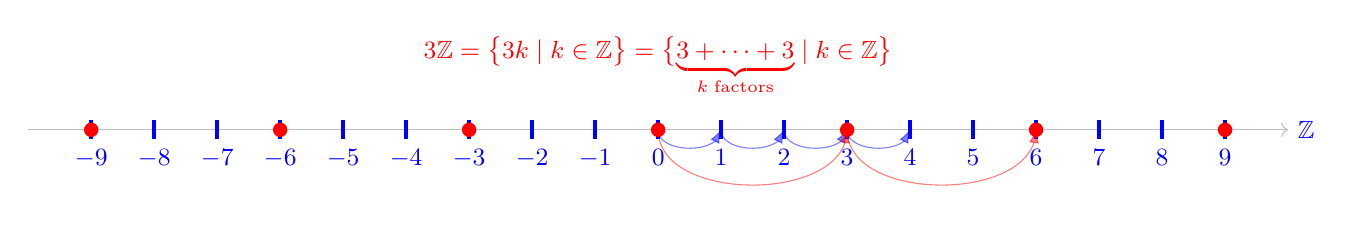
\begin{tikzpicture}[scale=.8, every node/.style={font=\small}]
		\draw[->, gray!50] (-10,0) -- (10,0);
		\node[right, blue] at (10,0) {$\mathbb{Z}$};
		
		\foreach \x in {-9,...,9} {
			\draw[blue, line width=.5mm] (\x,0.15) -- (\x,-0.15);
			\node[below, blue] at (\x,-0.15) {$\x$};
		}
	
		\draw[-Latex, bend angle=45, out=-90, in=-90, blue, opacity=.5] (0,0) to (1,0);
		\draw[-Latex, bend angle=45, out=-90, in=-90, blue, opacity=.5] (1,0) to (2,0);
		\draw[-Latex, bend angle=45, out=-90, in=-90, blue, opacity=.5] (2,0) to (3,0);
		\draw[-Latex, bend angle=45, out=-90, in=-90, blue, opacity=.5] (3,0) to (4,0);
		
		\def\n{3}
		\foreach \k in {-3,-2,-1,0,1,2,3} {
			\pgfmathsetmacro{\xcoord}{\k*\n}
			\filldraw[red] (\xcoord,0) circle (3pt);
		}
		\node[red, above] at (0,0.4) {$3\mathbb{Z}=\set{3k\mid k\in\Z}=\set[1]{\underbrace{3+\cdots+3}_{k\; \text{factors}}\mid k\in\Z}$};
		\draw[-Latex, bend angle=45, out=-90, in=-90, red, opacity=.5] (0,0) to (3,0);
		\draw[-Latex, bend angle=45, out=-90, in=-90, red, opacity=.5] (3,0) to (6,0);
		
	\end{tikzpicture}
	\end{center}
\end{observation}

\newpage
\begin{observation}[Partition via the Division Algorithm]
	Let $n\in\Z\setminus\set{0}$. Given any $a\in\Z$, the Division Algorithm guarantees that $\exists!q,r\in\Z$ such that \[
		a=nq+r,\quad\text{with $0\leq r< n$}.
	\] This leads to the relation $a-r=nq$, \ie, $a-r\in n\Z$. Consequently, we say that \[
	a+(-r)\in n\Z\iff n\mid a+(-r)\iff a\equiv r\pmod{n}.
	\] 
	\begin{center}
		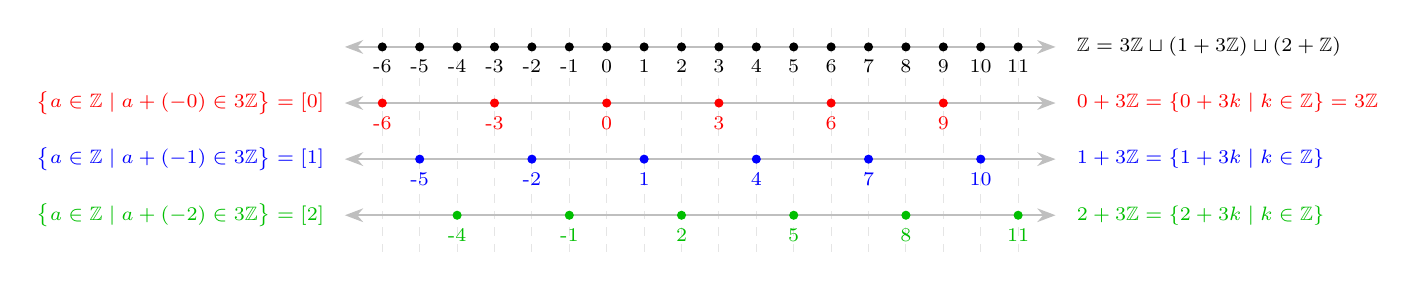
\begin{tikzpicture}[Stealth-Stealth,scale=.475, font=\scriptsize]
			% Dashed Line
			\foreach \x in {-6,-5,...,11} {
				\draw[-, dashed, gray!20] (\x, .5) -- (\x, -5.5);
			}
			% Z
			\draw[thick, gray!50] (-7,0) -- (12,0) node[font=\scriptsize, right=4pt,black] {$\Z=3\Z\sqcup(1+3\Z)\sqcup(2+\Z)$};
			\foreach \x in {-6,-5,...,11} {
				\filldraw (\x,0) circle (3pt);
				\node[below] at (\x,-.1) {\x};
			}
			% 3Z
			\draw[thick, gray!50] (-7,-1.5) -- (12,-1.5) node[font=\scriptsize, right=4pt, red] {$0+3\Z=\set[0]{0+3k\mid k\in\Z}=3\Z$};
			\node[font=\scriptsize, left=4pt, red] at (-7,-1.5) {$\set{a\in\Z\mid a+(-0)\in 3\Z}=[0]$};
			\foreach \x in {-6,-3,...,11} {
				\filldraw[red] (\x,-1.5) circle (3pt);
				\node[font=\scriptsize, below, red] at (\x,-1.6) {\x};
			}
			% 3Z + 1
			\draw[thick, gray!50] (-7,-3) -- (12,-3) node[font=\scriptsize, right=4pt, blue] {$1+3\Z=\set[0]{1+3k\mid k\in\Z}$};
			\node[font=\scriptsize, left=4pt, blue] at (-7,-3) {$\set{a\in\Z\mid a+(-1)\in 3\Z}=[1]$};
			\foreach \x in {-5,-2,...,11} {
				\filldraw[blue] (\x,-3) circle (3pt);
				\node[font=\scriptsize, below, blue] at (\x,-3.1) {\x};
			}
			% 3Z + 2
			\draw[thick, gray!50] (-7,-4.5) -- (12,-4.5) node[font=\scriptsize, right=4pt, green!75!black] {$2+3\Z=\set[0]{2+3k\mid k\in\Z}$};
			\node[font=\scriptsize, left=4pt, green!75!black] at (-7,-4.5) {$\set{a\in\Z\mid a+(-2)\in 3\Z}=[2]$};
			\foreach \x in {-4,-1,...,11} {
				\filldraw[green!75!black] (\x,-4.5) circle (3pt);
				\node[font=\scriptsize, below, green!75!black] at (\x,-4.6) {\x};
			}
		\end{tikzpicture}
	\end{center}
	Hence, one may assign to each $a\in\Z$ the corresponding set \begin{align*}
	a+n\Z&= (nq+r)+n\Z\\
	&=(r+nq)+n\Z \\
	&=r+n\Z=\set{r+nk:k\in\Z}.
	\end{align*} The set of all integers is the disjoint union of these residue classes: $\displaystyle\Z=\bigsqcup_{r=0}^{n-1}\left(r + n\Z\right)$.
\end{observation}
\vfill
\begin{note}
\ \begin{table}[h!]\centering
\begin{tabular}{l|lcl}
	{Group} & $(\Z,+)$ & & $(G,\ast)$ \\ \\
	{Subroup} & $(n\Z,+)\leq(\Z,+)$ & & $(H,\ast)\leq (G,\ast)$ \\ 
	\\
	{Relation} & $a\sim r\Leftrightarrow a+(-r)\in n\Z$& & $g_1\sim g_2\Leftrightarrow g_1\ast g_2^{-1}\in H$
	\\ 
	& & $\xrightarrow{\text{Generalization}}$ & \\
	{Coset} & $a+n\Z=\set[0]{a+nk:k\in\Z}$ & & $g\ast H:=\set[0]{g\ast h:h\in H}$ \\ \\
	{Quotient Group} & $\Z/n\Z=\set{a+n\Z:a\in\Z}$ with & & $G/H:=\set{g\ast H:g\in G}$ with \\
	{with Operation} & $(a+n\Z)\boxplus(b+n\Z):=(a+b)+n\Z$ & & $(g_1\ast H)\boxast(g_2\ast H):=(g_1\ast g_2)\ast H$\\ \\
	{Partition} & $\Z=\bigsqcup_{r=0}^{n-1}(r+n\Z)$ & & $G=\bigsqcup_{g\in G}(g\ast H)$
\end{tabular}
\end{table}
\end{note}

\newpage
\probox[]{\begin{proposition*}
	Let $(G,\ast)$ be a group and $H\leq G$. Define a binary relation $\sim_L$ and $\sim_R$ on $G$ by \begin{align*}
		g_1\sim_L g_2&\iff g_1^{-1}\ast g_2\in H,\\
		g_1\sim_R g_2&\iff g_1\ast g_2^{-1}\in H.
	\end{align*} 
	Then $\sim_L$ and $\sim_R$ are both equivalence relations on $G$.
\end{proposition*}}
\begin{proof}	
	We NTS that a relation $\sim_L$ on $G$ is reflexive, symmetric and transitive: \begin{enumerate}[(i)]
		\item (Reflexivity)\; Take $g\in G$. Note that $g^{-1}\ast g=e$ is the identity element of $G$. Since $H$ is a subgroup, it must contain $e$. Thus, $g^{-1}\ast g=e\in H,$ \ie, $g\sim_L g$.
		\item (Symmetry)\; Let $g_1,g_2\in G$. Suppose that $g_1\sim_L g_2$; that is, $g_1^{-1}\ast g_2\in H$. Since $H$ is a subgroup, \[
		g_2^{-1}\ast g_1=(g_1^{-1}\ast g_2)^{-1}\in H,\quad\ie,\quad g_2\sim_L g_1.
		\] 
		\item (Transitivity)\; Let $g_1,g_2,g_3\in G$. Suppose that $g_1\sim_L g_2$ and $g_2\sim_L g_3$; that is, $g_1^{-1}\ast g_2,g_2^{-1}\ast g_3\in H$. Since $H\leq G$, \[
		g_1^{-1}\ast g_3=g_1^{-1}\ast (g_2\ast g_2^{-1})\ast g_3=(g_1^{-1}\ast g_2)\ast (g_2^{-1}\ast g_3)\in H,\quad\ie,\quad g_1\sim_L g_3.
		\]
	\end{enumerate} Hence, $\sim_L$ is equivalence relations on $G$ and similarly $\sim_R$ is also.
\end{proof}
\vfill
\defbox[Coset]{\begin{definition*}
Let \( (G,\ast) \) be a group with identity element \( e \), and let $
H \leq G$ be a subgroup of \( G \). For any element \( g \in G \), the \textbf{left coset} of \( H \) in \( G \) corresponding to \( g \) is defined by \[
g\ast H \coloneqq \{\, g \ast h : h \in H \,\}\subseteq G.
\]
Similarly, the \textbf{right coset} of \( H \) in \( G \) corresponding to \( g \) is defined by $
H\ast g \coloneqq \{\, h \ast g : h \in H \,\}.$
\end{definition*}}
%\begin{remark*}
%	The term coset is used to emphasize that these subsets of $G$ arise by the process of "translating" the subgroup $H$ by an element $G$ of $G$. In particular, the coset $gH$ is the image of $H$ under the left-multiplication map \[
%	L_g:G\to G,\quad L_g(h)=g\ast h
%	\]
%	Thus, cosets can be understood as the ``shifted copies'' of $H$ within the group $G$.
%\end{remark*}
\begin{remark*}
	Note that \[
	x\in g\ast H\iff\exists h\in H; \text{such that}\;x=g\ast h.
	\] Thus, $H=e\ast H=H\ast e$ since $h=e\ast h=h\ast e$ for any $h\in H$.
\end{remark*}
\begin{remark*}
	Consider the equivalence relation $\sim_L$ on $G$. For each $g\in G$, we obtain \[
	[g]=\set{x\in G: g\sim_L x}=\set[1]{x\in G:g^{-1}\ast x\in H}=\set{g\ast h:h\in H}=gH.
	\]
\end{remark*}
\newpage
\probox[Coset Equality Criterion]{\begin{proposition*}
	Let $G$ be a group and let $H\leq G$ be a subgroup. Then, for all $g_1,g_2\in G$, the following conditions are equivalent: \begin{enumerate}[(1)]
		\item $g_1\ast H=g_2\ast H$\;
		\item $g_1^{-1}\ast g_2\in H$\;
		\item $g_2^{-1}\ast g_1\in H$.
	\end{enumerate}
\end{proposition*}}
\begin{proof}
	Let $g_1,g_2\in G$. \\
	\ \\
	\text{[(1)$\Rightarrow$(2)]}\; Assume that $g_1\ast H=g_2\ast H$. Then \begin{align*}
		g_2=g_2\ast e\implies g_2\in g_2H=g_1H &\implies \exists h\in H\; \text{s.t.}\; g_2=g_1\ast h\\
		&\implies g_1^{-1}\ast g_2=h\in H.
	\end{align*}
	\text{[(2)$\Rightarrow$(1)]}\; Assume that $g_1^{-1}\ast g_2\in H=e\ast H$. Then \[
	\exists h\in H\;\text{such that}\; g_1^{-1}\ast g_2=e\ast h=h,\; \ie,\; g_2=g_1\ast h.
	\]\par
	(a) ($g_1H\supseteq g_2H$)\; Let $y\in g_2\ast H$ then $\exists h'\in H\; \text{such that}\; y=g_2\ast h'$. Thus \[
	y=g_2\ast h'=(g_1\ast h)\ast h'=g_1\ast (h\ast h')\overset{h\ast h'\in H}{\in} g_1H.
	\]\par
	(b) ($g_1H\subseteq g_2H$)\; Let $x\in g_1\ast H$ then $\exists h''\in H\; \text{such that}\; x=g_1\ast h''$. Thus \[
	x=g_1\ast h''=(g_2\ast h^{-1})\ast h''=g_2\ast (h^{-1}\ast h'')\overset{h^{-1}\ast h'\in H}{\in} g_2\ast H.
	\] By (a) and (b), we obtain that $g_1\ast H=g_2\ast H$.
	\\ \ \\
	\text{[(2)$\Leftrightarrow$(3)]}\; Note that $(g_1^{-1}g_2)^{-1}=g_2^{-1}g_1$. Since $H$ is a subgroup, we have \[
	g_1^{-1}g_2\in H\iff (g_1^{-1}g_2)^{-1}\in H\iff g_2^{-1}g_1\in H.
	\]
\end{proof}
\newpage
\probox[Equal Cardinalities of Cosets]{\begin{proposition*}
	Let $(G,\ast)$ be a group, and let $H\leq G$. Then \[
	\abs[0]{g\ast H}=\abs[0]{H},\quad\text{for all}\; g\in G.
	\]
\end{proposition*}}
\begin{proof}
Let $g\in G$. Define a mapping \[
\varphi:H\to g\ast H,\quad h\mapsto \varphi(h):=g\ast h.
\] We NTS that $\varphi$ is a bijection: \begin{enumerate}[(i)]
	\item (Injectivity)\; Let $h_1,h_2\in H$. Then \begin{align*}
		\varphi(h_1)=\varphi(h_2) &\implies g\ast h_1= g\ast h_2\\
		&\implies g^{-1}\ast (g\ast h_1)=g^{-1}\ast(g\ast h_2)\\
		&\implies h_1=h_2.
	\end{align*}
	\item (Surjectivity)\; Let $x\in g\ast H$. Then $\exists h\in H$ such that $x=g\ast h$, and so \[
	\varphi(h)=g\ast h=x.
	\]
\end{enumerate} Hence it is proved.
\end{proof}

\newpage
\defbox[Quotient Group $G/H$]{\begin{definition*}
		Let $G$ be a group and let $H$ be a \text{\color{gray!50}normal} subgroup of $G$ {\color{gray!50}(that is, $g\ast H\ast g^{-1}=H$ for all $g\in G$)}. The \textbf{quotient group} $G/H$ is defined by \[
		G/H:=\set{g\ast H:g\in G},
		\] where for each $g\in G$, the \emph{left coset} $g\ast H$ is the set \[
		g\ast H:=\set{g\ast h:h\in H}.
		\] The binary operation on $G/H$ is defined by \[
		(g_1\ast H)\boxast(g_2\ast H):=(g_1\ast g_2)\ast H,\quad\text{for all}\; g_1,g_2\in G.
		\]
\end{definition*}}
\begin{exercise*}
	Prove that there exists a group isomorphism from $G/\set{e}$ to $G$.
	\begin{proof}[\sol]
		The set of left cosets of $\set{e}$ in $G$ is $G/\set{e}=\set{g\ast\set{e}:g\in G}$. Define a function \[
		\varphi:G/\set{e}\to G,\quad g\ast\set{e}\mapsto\varphi(g\ast\set{e}):=g.
		\] Then \begin{enumerate}[(i)]
			\item (Well-definedness)\; Let $g\ast\set{e}=h\ast\set{e}$ for some $g,h\in G$. Then \[
			h^{-1}\ast g\in\set{e}\implies h^{-1}\ast g=e\implies g=h.
			\]
			\item (Homomorphism)\; Let $g\ast\set{e},h\ast\set{e}\in G/\set{e}$. Then \[
			\varphi((g\ast\set{e})\boxast(h\ast\set{e}))=\varphi((g\ast h)\ast\set{e})=g\ast h=\varphi(g\ast\set{e})\ast \varphi(h\ast\set{e})
			\]
			\item (Injectivity)\; $\varphi(g\ast\set{e})=\varphi(h\ast\set{e})\implies g=h\implies g\ast\set{e}=h\ast\set{e}$.
			\item (Surjectivity)\; Let $g\in G$. Then $\exists g\ast\set{e}\in G/\set{e}$ such that $\varphi(g\ast\set{e})=g$.
		\end{enumerate}
	\end{proof}
\end{exercise*}

\newpage
\thmbox[Lagrange’s Theorem]{\begin{theorem*}
	Let $(G,\ast)$ be a finite group and let $H\leq G$ be a subgroup. Then \[
	\abs{H}\quad\text{divides}\quad\abs{G}.
	\]
\end{theorem*}}
\begin{proof}
%Recall that \begin{enumerate}
%	\item (Partition of $G$ via an Equivalence Relation)\; Define a relation \(\sim_L\) on \(G\) by \[
%	g_1 \sim g_2 \iff g_1^{-1}\ast g_2 \in H.
%	\] Then \(\sim_L\) be an equivalence relation on \(G\). Its equivalence class containing \(g \in G\) is given by \[
%	[g] = \{ x \in G : g^{-1}\ast x \in H \} = \{ g\ast h : h \in H \} = g\ast H.
%	\] The collection of equivalence classes $\set{g\ast H}_{g\in G}$ forms a partition of $G$, \ie, $G=\bigsqcup_{g\in G}(g\ast H)$.
%	\item (Equal Cardinalities of Cosets)\; Let \(g \in G\). Consider the mapping\[
%	\varphi : H \to g\ast H, \quad h\mapsto \varphi(h) = g\ast h.
%	\]
%	Since $\varphi$ is a group isomorphism, it follows that $\abs[0]{g\ast H}=\abs[0]{H}$.
%\end{enumerate}
Consider equivalence classes (left cosets) be denoted by \[
g_1H,\; g_2H,\; \dots,\; g_kH,
\] where \(k\in\N\). Since $
G = \bigsqcup_{i=1}^{k} g_iH$, we have \begin{align*}
	|G| &= \sum_{i=1}^{k} |g_iH|\\
	&=\sum_{i=1}^{k} |H|\quad\because \abs[0]{g_iH}=\abs[0]{H}\quad\text{for all}\; i=1,2,\dots,k. \\
	&= k\cdot |H|.
\end{align*} Hence, the order (cardinality) of $H$ divides the order of $G$.
\end{proof}
%\vfill
%\begin{remark*}
%	Let $G$ be a finite group and let $H\leq G$ be a subgroup. Then by Lagrange's Theorem, \[
%	\exists k\in \Z\;\text{such that}\; \abs{G}= k\cdot\abs{H}.
%	\] Here, the integer $k$ is called the \textbf{index} of $H$ in $G$, denoted by $[G:H]$, is defined by \[
%	[G:H]:=\frac{\abs{G}}{\abs{H}},\quad \ie,\quad \abs{G}=[G:H]\cdot\abs{H}. 
%	\]
%\end{remark*}
\vfill
\corbox{\begin{corollary*}
		Let $p$ be a prime. Then $\Z/p\Z$ has no proper subgroup except $\set{e}$. In other words, if $H$ is a subgroup of $\Z/p\Z$, then either \[
		H=\set{[0]}\quad\text{or}\quad H=\Z/p\Z.
		\]
\end{corollary*}}
\begin{proof}
	Consider the group \( G = \mathbb{Z}/p\mathbb{Z} \). Since \( p \) is prime, we have $|G| = p$.
	Let \( H\leq\mathbb{Z}/p\mathbb{Z} \). Then, by Lagrange’s Theorem, \( |H| \) must divide \( p \). By the definition of a prime, \[
	|H| \in \{1, p\}.
	\]
	\textbf{Case 1.}\; If \( |H| = 1 \), then \( H = \{[0]\} \).\\
	\textbf{Case 2.}\; If \( |H| = p \), then \( H = \mathbb{Z}/p\mathbb{Z} \).\\ \ \\
	Thus, there is no proper nontrivial subgroup of \(\mathbb{Z}/p\mathbb{Z}\); the only subgroups are the trivial subgroup and the group itself.
	%Since \(\mathbb{Z}/p\mathbb{Z}\) is a cyclic group of order \(p\) (with \([1]\) as a generator), every subgroup of \(\mathbb{Z}/p\mathbb{Z}\) is cyclic. Let \( H \leq \mathbb{Z}/p\mathbb{Z} \) be a subgroup. We consider two cases:
	%\ \\ \ \\
	%\textbf{Case 1.} ($H$ is trivial) Clearly, \( H = \{[0]\} \).
	%\ \\ \ \\
	%\textbf{Case 2.}  ($H$ is nontrivial)\; Let \([a]\in H\) with \([a] \neq [0]\). Since \( H \) is cyclic, \[
	%H = \langle [a] \rangle.
	%\] By Lagrange's Theorem, $\ord([a])$ divides $\abs[0]{\Z/p\Z}=p$. However, since \(p\) is prime and \([a] \neq [0]\), \[
	%\operatorname{ord}([a]) = p.
	%\]
	%Hence, \(\langle [a] \rangle\) contains \(p\) distinct elements and therefore
	%\[
	%H = \langle [a] \rangle = \mathbb{Z}/p\mathbb{Z}.
	%\]
	%Thus, every subgroup \(H\) of \(\mathbb{Z}/p\mathbb{Z}\) is either \(\{[0]\}\) or \(\mathbb{Z}/p\mathbb{Z}\).
\end{proof}
\newpage
\corbox{\begin{corollary*}
	Every group of prime order is cyclic.
\end{corollary*}}
\begin{proof}
	Let $|G| = p$, where p is prime. Then $|G| > 1$ and so $\exists g\in G$ with $g\neq e$. Consider $\cyclic{g}\leq G$. By Lagrange’s Theorem,\; $\abs[0]{\cyclic{g}}$ divides $\abs[0]{G}=p$. Since 
	$p$ is prime, either \[
	\ord(g)=1\quad\text{or}\quad\ord(g)=p.
	\]
	\textbf{Case 1.}\; If \( \ord(g) = 1 \), then \( G = \{e\}\). It is contradict to the $\abs{G}>1$.\\
	\textbf{Case 2.}\; If \( \ord(g) = p \), then \( \abs{G}=p=\abs{\cyclic{g}}\).\\ \ \\
%	Conse-
%	quently, hai ≤ G has at least two elements, a and e. By the Lagrange’s theorem, the order m > 1 of
%	hai satisfies m | p. Since p is prime, m = p and hai = G, so G is cyclic.
	Therefore, $G=\cyclic{g}$.
\end{proof}

\vfill
\begin{thebibliography}{9}
	\bibitem{abstract_algebra_a}
	수학의 즐거움, Enjoying Math. ``수학 공부, 기초부터 대학원 수학까지, 20. 추상대수학 (a) 순환군의 분류 Classification of cyclic group'' YouTube Video, 22:01. Published 
	October 18, 2019. URL: \url{https://www.youtube.com/watch?v=1yQ52OSB_Cc&t=708s}.
	\bibitem{abstract_algebra_b}
	수학의 즐거움, Enjoying Math. ``수학 공부, 기초부터 대학원 수학까지, 21. 추상대수학 (b) 순환군과 라그랑지 정리의 역방향 cyclic group and inverse of Lagrange theorem'' YouTube Video, 32:03. Published 
	October 19, 2019. URL: \url{https://www.youtube.com/watch?v=_oY-2n6_xEg&t=1744s}.
	\bibitem{abstract_algebra_c}
	수학의 즐거움, Enjoying Math. ``수학 공부, 기초부터 대학원 수학까지, 22. 추상대수학 (c) 잉여류와 라그랑지 정리 set of cosets and Lagrange's theorem'' YouTube Video, 22:33. Published 
	October 22, 2019. URL: \url{https://www.youtube.com/watch?v=dsyssRBSqow&t=835s}.
\end{thebibliography}

\newpage
\appendix
\section{Number Theory}

\subsection{Divisibility}
\defbox[Divisibility]{\begin{definition*}
	Let $a,b\in\Z$ with $a\neq 0$. Then $a$ \textbf{divides} $b$ if \[
	\exists c\in\Z\quad\text{such that}\quad b=ac.
	\] Then $a$ is \emph{divisor} or \emph{factor} of $b$ and $b$ is \emph{multiple} of $a$.
\end{definition*}}
\begin{remark*}
	We write $a\mid b$ if $a$ divides $b$, and $a\nmid b$ otherwise. 
%	That is, \begin{align*}
%		a\mid b&\iff\exists c\in\Z\;\text{such that}\; b=ac\\
%		a\nmid b&\iff\forall c\in\Z,\; b\neq ac.
%	\end{align*}
\end{remark*}
\begin{remark*}
	Let $a,b\in\N$. Then $a\mid b\implies a\leq b$.
	\begin{proof}	
		Let \(a \mid b\). Then \[
		\exists k\in\N\quad\text{such that}\quad b = a\cdot k.
		\] Note that \(k \ge 1\). Then \[
		a\cdot k\geq a\cdot 1\implies b\geq a\cdot 1\implies b\geq a.
		\]
	\end{proof}
\end{remark*}
\vfill
\probox[]{\begin{proposition*}
	Let $a,b,c\in \Z$. \begin{enumerate}[(1)]
		\item $a\mid b$ and $b\mid c\implies a\mid c$.
		\item Let $c\neq 0$. Then $ca\mid cb\implies a\mid b$.
	\end{enumerate}
\end{proposition*}}
\begin{proof}
	Let $a,b,c\in\Z$. \begin{enumerate}[(1)]
		\item Let $a\mid b$ and $b\mid c$. Then $\exists u, v\in\Z\;\text{s.t.}\; au=b\;\text{and}\; bv=c$. Thus $$c=bv=(au)v=a(uv),$$ and so $a\mid c$.
		\item Let $ca\mid cb$ with $c\neq 0$. Then $\exists u\in\Z$ s.t. $cb=cau$. Hence $b=au$, and so $a\mid b$.
	\end{enumerate}
\end{proof}

\newpage
\probox[]{\begin{proposition*}
	Let $a,b,c\in \Z$. For any $m,n\in\Z$, \[
	c\mid a\;\text{and}\; c\mid b\implies c\mid (ma+nb).
	\]
\end{proposition*}}
\begin{proof}
	Let $m.n\in\Z$, and let $a\mid b$ and $b\mid c$. Then \[
	\exists e, f\in\Z\;\text{such that}\; a=ce\;\text{and}\; b=cf.
	\] Hence \[
	ma+nb=m(ce)+n(cf)=c(me+nf),
	\] and so $c\mid (ma+nb)$.
\end{proof}
\vspace{50pt}
\thmbox[Euclid's Lemma]{\begin{theorem*}
	\hypertarget{euclid_lemma}{}
	Let $a,b,c\in\Z$, and let $a\mid bc$. Then \[
	\gcd(a,b)=1\implies a\mid c.
	\]
\end{theorem*}}
\begin{proof}
By Bézout's Identity, \( \exists a,b\in\mathbb{Z} \) such that \[
ax+by=\gcd(a,b)=1.
\] Consider \[
c\cdot 1= c(ax+by)=cax+cby.
\] Since $a\mid ac$ and $a\mid bc$, we have \[
a\mid (cax+cby).
\] Hence, $a\mid c$.
\end{proof}
\newpage
\subsection{Modular Arithmetic}
\defbox[Congruence (Number Theory)]{\begin{definition*}
	Let $n$ be a positive integer ($n\in\N$). Two integers 
	$a$ and  $b$ are said to be \textbf{congruent modulo $n$}, written as
	\[
	a\equiv b\pmod{n},
	\] if and only if \[
	n\mid a-b,\quad\ie,\quad \exists k\in\Z\; \text{such that}\; a-b=kn.
	\]
\end{definition*}}
\begin{remark*}[Modulo Operation]
According to the \textbf{division algorithm}, for any integer 
$a$ and any positive integer $n$, there exist unique integers 
$q$ (the quotient) and $r$ (the remainder) such that \[
a=qn+r\quad\text{with}\quad 0\leq r< n.
\] When we express this using the floor function and the mod operation, we identify: \[
q=\floor*{\frac{a}{n}}\quad\text{and}\quad r= a\bmod n.
\] Thus,  we can rewrite the division algorithm as: \[
a=n\floor*{\frac{a}{n}}+(a\bmod n).
\] Thus, we have \[
a\bmod n:=\begin{cases}
	\displaystyle a-n\floor*{\frac{a}{n}} &: n\neq 0\\
	\displaystyle 0 &: n= 0.
\end{cases}
\] Note that \[
a\equiv b\pmod{n}\iff a\bmod n=b\bmod n.
\]
\end{remark*}

\subsection{Greatest Common Divisors}
\defbox[Greatest Common Divisor; GCD]{\begin{definition*}
	Let $a,b\in \Z$. An nonnegative integer $d\in\Z_{\geq 0}$ is called a \textbf{greatest common divisor (gcd)} of $a$ and $b$, denoted by $d=\gcd(a,b)$, if it satisfies the following two conditions: \begin{enumerate}[(i)]
		\item (Divisibility)\; $d\mid a$ and $d\mid b$.
		\item (Maximality)\; For any $c\in\Z$, \[
		c\mid a\; \text{and}\; c\mid b\implies c\mid d.
		\]
	\end{enumerate}
\end{definition*}}
\vfill
\probox{\begin{proposition*}
	Let $a,b,c\in \Z$. \begin{enumerate}[(1)]
		\item $\gcd(a+cb,b)=\gcd(a,b)$.
		\item $\displaystyle\gcd(a,b)=d\implies \gcd\left(\frac{a}{d},\frac{b}{d}\right)=1$.
	\end{enumerate}
\end{proposition*}}
\begin{proof}
	TBA
\end{proof}
\vfill
%\newpage
\thmbox[Bezout's Identity]{\begin{theorem*}
	Let $a,b\in\Z$. Then \[
	\exists m,n\in\Z\quad\text{such that}\quad \gcd(a,b)=ma+mb.
	\]
\end{theorem*}}
\begin{remark*}
	Note that there are infinitely many such $m$ and $n$.
\end{remark*}
\begin{proof}
	It is proved by well-ordering principle.
\end{proof}


\corbox{\begin{corollary*}
	Let $a,b\in\Z$. \[
	\gcd(a,b)=1\implies \exists m,n\in\Z\;\ \text{such that}\; ma+nb=1.
	\]
\end{corollary*}}

\newpage
\subsection{Prime Number}
\defbox[Prime Number]{\begin{definition*}
	A number $p\in\N_{>1}$ is \textbf{prime} if, for $m>0$, \[
	m\mid p\implies m=1\;\text{or}\; m=p.
	\] A number which is not prime is composite.
\end{definition*}}
\begin{remark*}
	A number $p\in\N_{>1}$ is \textbf{prime} if, for $m>0$, $m\mid p\implies m\in\set{1,p}$.
\end{remark*}

\end{document}
